\documentclass[12pt, a4paper]{ctexart} % 直接使用中文文档类

% ---------- 页面设置 ----------
\usepackage{algorithm}      % 算法环境
\usepackage{algorithmic}    % 算法伪代码
\usepackage{amsmath}        % 数学公式支持
\usepackage{geometry}
\usepackage{indentfirst}   % 让首段也缩进
\usepackage{graphicx}
\usepackage{amsfonts} % 或者使用 \usepackage{amssymb}////为了使用黑体字公式
\usepackage{booktabs}%三线表格式

\setlength{\parindent}{2em} % 缩进2字符(1em≈1汉字宽度)
\geometry{left=3cm, right=2.5cm, top=2.5cm, bottom=2.5cm}

% ---------- 字体配置 ----------
\setmainfont{Times New Roman}          % 设置西文字体

% ---------- 段落格式 ----------
\linespread{1.5}                      % 1.5倍行距
\setlength{\parindent}{2em}           % 首行缩进

% ---------- 标题格式 ----------
\usepackage{titlesec}
\titleformat{\section}{\Large\bfseries\heiti}{\thesection}{1em}{}
\titleformat{\subsection}{\large\bfseries\heiti}{\thesubsection}{1em}{}

% ---------- 文档信息 ----------
\title{使用随机森林估计和推断异质性治疗效果}
\author{译者 Tinkle}
\date{\today}

\begin{document}
\maketitle{}
% ---------- 摘要页 ----------
\begin{abstract}
    尽管被广泛的采用,机器学习模型大多是黑匣子。然而,了解预测背后的原因对于评估信任非常重要,如果一个人计划根据预测采取行动,或者在选择是否部署新模型时,这一点至关重要。这种理解还提供了对模型的见解,可用于将不可信的模型或预测转换为可信的模型或预测。
    
    在这项工作中,我们提出了 LIME,这是一种新颖的解释技术,通过围绕预测在本地学习可解释模型,以可解释和忠实的方式解释任何分类器的预测。我们还提出了一种解释模型的方法,通过以非冗余的方式呈现具有代表性的单个预测及其解释,将任务构建为子模优化问题。我们通过解释文本(例如随机森林)和图像分类(例如神经网络)的不同模型来展示这些方法的灵活性。我们通过模拟和人类受试者的新颖实验来展示解释在各种需要信任的场景中的效用:决定是否应该相信预测、在模型之间进行选择、改进不可信的分类器以及确定为什么不应该信任分类器。
\end{abstract}

% ---------- 正文部分 ----------
\section{引言}
机器学习是许多最新科学和技术进步的核心。不幸的是,人类的重要作用是该领域经常被忽视的一个方面。无论人类是直接使用机器学习分类器作为工具,还是在其他产品中部署模型,一个至关重要的问题仍然存在:如果用户不信任模型或预测,他们就不会使用它。区分信任的两种不同(但相关)定义很重要:(1) 信任预测,即用户是否足够信任单个预测以根据它采取一些行动,以及 (2) 信任模型,即用户是否相信模型在部署后会以合理的方式运行。

两者都收到人类对模型行为的理解程度,而不是将其视为黑匣子。当模型用于决策时,确定对单个预测的信任度是一个重要问题。例如,当使用机器学习进行医疗诊断 [6] 或恐怖主义侦查时,不能盲目相信地进行预测,因为后果可能是灾难性的。

除了信任单个预测之外,还需要在“野外”部署模型之前将其作为一个整体进行评估。要做出此决定,用户需要确信该模型将根据感兴趣的指标在实际数据上表现良好。目前,模型使用可用验证数据集上的准确率指标进行评估。但是,实际数据通常存在显著差异,此外,评估指标可能并不表示产品的目标。除了此类指标之外,检查单个预测及其解释也是一种有价值的解决方案。在这种情况下,通过建议要检查的实例来帮助用户非常重要,尤其是对于大型数据集。

在本文中,我们建议为单个预测提供解释作为 “信任预测 ”问题的解决方案,并选择多个这样的预测 (和解释) 作为 “信任模型 ”问题的解决方案。我们的主要贡献总结如下。

LIME,一种可以通过使用可解释模型进行局部近似来忠实地解释任何分类器或回归器的预测的算法。

SP-LIME,一种通过子模优化选择一组具有代表性实例并附有解释来解决“信任模型”问题的方法。

对模拟和人类受试者进行综合评估,我们衡量解释对信任和相关任务的影响。在我们的实验中,使用 LIME 的非专家能够从一对分类器中选择哪个分类器在现实世界中泛化得更好。此外,通过使用 LIME 进行特征工程,他们能够大大改进在 20 个新闻组上训练的不可信分类器。我们还展示了了解神经网络对图像的预测如何帮助从业者了解何时以及为什么不应该信任模型。

\section{解释的理由}
“解释预测”是指呈现文本或视觉工件,这些工件提供了对实例组件(例如文本中的单词、图像中的补丁)与模型预测之间关系的定性理解。我们认为,解释预测是让人类信任并有效使用机器学习的一个重要方面,前提是解释要忠实、易懂。

\begin{figure}[h]
    \centering
    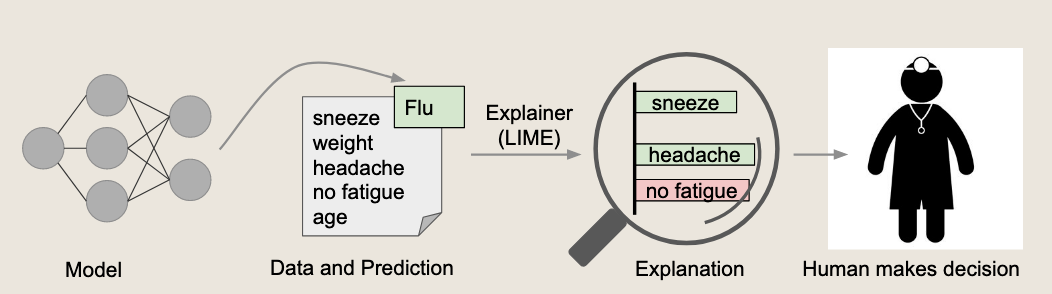
\includegraphics[width=0.6\textwidth]{img/img_1.png}
    \caption{解释单个预测。模型预测患者患有流感,而 LIME 会突出显示患者病史中导致预测的症状。打喷嚏和头痛被描绘成有助于 “流感 ”预测,而 “没有疲劳 ”则是反对它的证据。有了这些,医生可以就是否信任模型的预测做出明智的决定。}
    \label{fig:img_1}
\end{figure}
